\newpage
\section{Catalog}

\begin{figure}[ht]
	\centering
  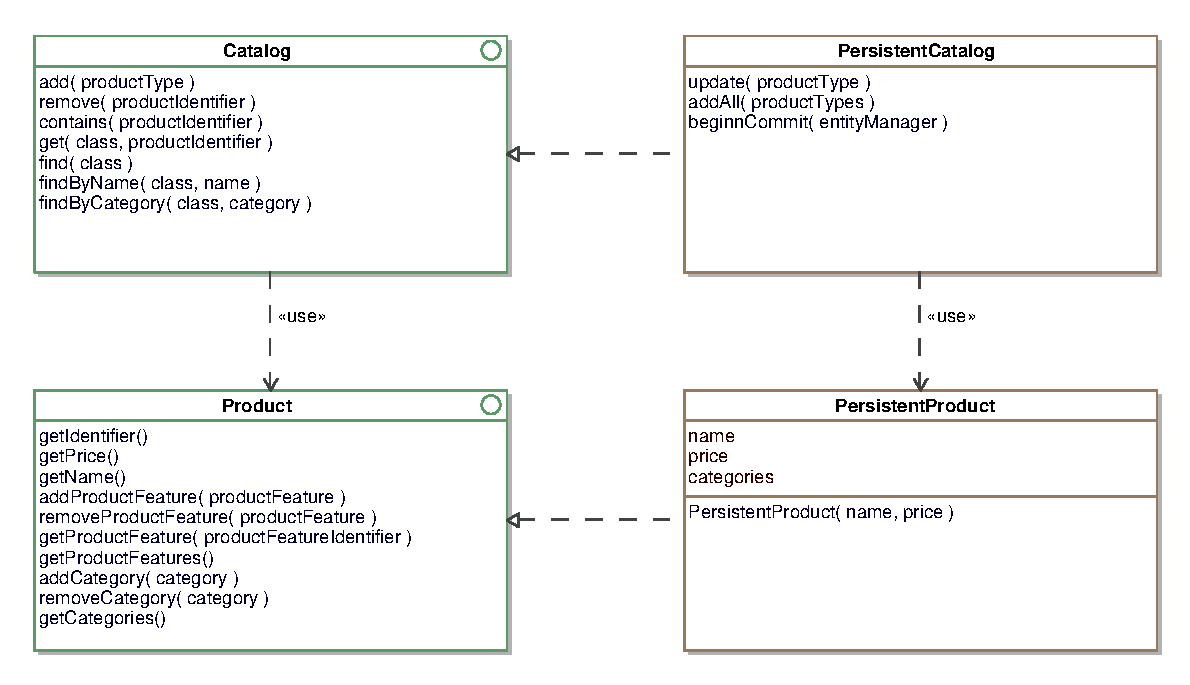
\includegraphics[width=1.0\textwidth]{images/Catalog_Overview.eps}
	\label{catalog_overview}
	\caption{Catalog - Class Overview}
\end{figure}

\subsection{\code{Catalog} - Organizing and presenting \code{ProductTypes}}
\code{Catalog} is an interface and provides methods for adding and removing \code{ProductTypes} as well as finding them based on the \code{ProductType} via its name and category.
\code{PersistentCatalog} is an implementation of the \code{Catalog}-interface and provides the \code{update(PersistentProductType productType)} method for updating and persisting an existing \code{PersistentProductType} to the \code{PersistentCatalog} and the database. 
Every operation is delegated to the database, via \code{CriteriaQuery}s. Some methods require additional processing of query results with Java.
\code{Catalog} aggregates \code{ProductType}s, \code{PersistentCatalog} aggregates \code{PersistentProductType}s.




%If you want to sell your products at your shop, you must presenting them very good to stimulate customers interests. A helpful solution to giving this people a clearly overview could be
%a catalog. With the \code{PersistentCatalog}-class, you can implemented such a thing. This class is an implementation of the interface \code{Catalog}.\\
%After you created a new catalog, you can add \code{ProductTypes} to it or remove them from it. Also you can checked, whether the catalog contains a defined \code{ProductType}. Aside from you 
%this class provides methods to find productTypes by their name or their category at your catalog.\\
%In case you have added a \code{ProductType} to the catalog and now you are changing this type, you do not need remove the old type from this catalog and add the new to it. Only you need to 
%used the method \code{update(PersistentProductType productType)} from the \code{PersistentCatalog}-class and this \code{productType} will be updated and persist to the \code{PersistentCatalog} 
%and the Database.

